\chapter{Linear Optics}

%-----------------------------------------------------------------
\section{Coupling and Normal Modes}
\label{s:coupling}
\index{normal mode!Coupling}

The coupling formalism used by \bmad is taken from the paper of Sagan and Rubin\cite{b:coupling}.
The main equations are reproduced here.

The analysis starts with the map $\bfT(s)$ for the transverse two--dimensional phase space
coordinates $\bfx = (x, x', y, y')$. In ring, with a closed geometry, this map will be a one-turn
map starting and ending at some point $s$. For a machine with open geometry, $\bfT(0)$ can be
computed from the initial Twiss and coupling parameters and $\bfT(s)$ can then be computed by
propagating with the transfer map $\bfM_{0s}$ from $0$ to $s$:
\begin{equation}
    \bfT(s) = \bfM_{0s} \, \bfT(0) \, \bfM_{0s}^{-1}
\end{equation}

\index{normal mode!a--mode}
\index{normal mode!b--mode}
$\bfT$ can be decomposed using a similarity transformation
 can be written as
  \begin{equation}
    \bfT = \bfV \, \bfU \, \bfV\inv 
    , \label{tvuv}
  \end{equation} 
where $\bfV$ is symplectic, and $\bfU$ is of the form
  \begin{equation}
    \bfU =
    \begin{pmatrix}
      \bfA & \Bf0 \cr 
      \Bf0 & \bfB \cr
    \end{pmatrix}
    . \label{ua00b}
  \end{equation}
Since $\bfU$ is uncoupled, the standard Twiss analysis can be performed with the $\bfA$ and $\bfB$
matrices being parameterized using the standard form:
\begin{equation}
  \bfA = \begin{pmatrix}
    \cos\theta_a + \alpha_a \, \sin\theta_a & \beta_a \, \sin\theta_a \\
    -\gamma_a \, \sin\theta_a & \cos\theta_a - \alpha_a \, \sin\theta_a
    \end{pmatrix}
\end{equation}
with a similar equation for $\bfB$. 

The $\bfV$ ``coupling'' matrix is written in the form:\footnote
  {
The form of $\bfV$ and $\bfU$ is not unique. The form of $\bfV$ and $\bfU$ used here essentially
follows the form given by Edwards and Teng\cite{b:edteng}.
  }
  \begin{equation}
    \bfV = 
    \begin{pmatrix}
        \gamma \bfI & \bfC \cr 
        -\bfC^+     & \gamma \bfI \cr
    \end{pmatrix}
    , \label{vgicc1}
  \end{equation}
where $\bfC$ is a 2x2 matrix and $+$ superscript denotes the symplectic conjugate:
\index{symplectic!conjugate}
  \begin{equation}
    \bfC^+ = 
    \begin{pmatrix}
       C_{22} & -C_{12} \cr 
      -C_{21} & C_{11} \cr
    \end{pmatrix}
    . \label{ccccc}
  \end{equation}
Since we demand that $\bfV$ be symplectic we have the condition
  \begin{equation}               
    \gamma^2 + \, |\bfC| = 1
    , \label{gc1}
  \end{equation}
and $\bfV\inv$ is given by
  \begin{equation}
    \bfV\inv = 
    \begin{pmatrix}
      \gamma \bfI & -\bfC \cr 
      \bfC^+ & \gamma \bfI \cr
    \end{pmatrix}
    . \label{vgicc2}
  \end{equation} 
$\bfC$ is a measure of the coupling. $\bfT$ is uncoupled if and only if $\bfC = \Bf 0$.

It is useful to normalize out the $\beta(s)$ variation in the above analysis. Normalized quantities
being denoted by a bar above them. The normalized normal mode matrix $\BAR\bfU$ is defined by
  \begin{equation}
    \BAR\bfU = \bfG \, \bfU \, \bfG\inv
    , \label{ugug}
  \end{equation}
Where $\bfG$ is given by 
  \begin{equation}
    \bfG \equiv 
    \begin{pmatrix}
      \bfG_a & \Bf0 \cr 
      \Bf0 & \bfG_b
    \end{pmatrix}
    , \label{gg00g}
  \end{equation}  
with 
  \begin{equation}
    \bfG_a = 
    \begin{pmatrix}
      \frac{\tstyle 1}{\tstyle \sqrt{\beta_a}} & 0 \cr
      \frac{\tstyle \alpha_a}{\tstyle \sqrt{\beta_a}} & \sqrt{\beta_a}
    \end{pmatrix}
    , \label{g1b0a} 
  \end{equation}
with a similar equation for $\bfG_b$. With this definition, the corresponding $\BAR\bfA$ and
$\BAR\bfB$ (cf.~\Eq{ua00b}) are just rotation matrices. The relationship between $\bfT$ and
$\BAR\bfU$ is
  \begin{equation}
    \bfT = \bfG\inv \, \BAR\bfV \, \BAR\bfU \, \BAR\bfV\inv \, \bfG
    , \label{tgvuv}
  \end{equation}
where
  \begin{equation}
    \BAR\bfV = \bfG \, \bfV \, \bfG\inv
    . \label{vgvg}
  \end{equation}
Using \Eq{gg00g}, $\BAR\bfV$ can be written in the form
  \begin{equation}
    \BAR\bfV = 
    \begin{pmatrix}
      \gamma \bfI & \BAR\bfC \cr -\BAR\bfC^+ & \gamma \bfI
    \end{pmatrix}
    , \label{vgicc3}
  \end{equation}
with the normalized matrix $\BAR\bfC$ given by
  \begin{equation}
    \BAR\bfC = \bfG_a \, \bfC \, \bfG_b\inv
    . \label{cgcg}
  \end{equation}

The two normal modes of oscillation are denoted $a$ and $b$ with the $a$-mode associated with the
$\bfA$ matrix and the $b$-mode associated with the $\bfB$ matrix. The normal mode phase space
coordinates are denoted ${\bf a} = (a, p_a, b, p_b)$. If the one--turn matrix $\bfT$ is uncoupled
then the $a$-mode is associated with horizontal horizontal motion and $b$-mode is associated with
vertical motion.

The normal mode coordinates ${\bf a}$ are related to the laboratory frame via
  \begin{equation}
    {\bf a} = \bfV\inv \, {\bf x}
    . \label{avx}
  \end{equation} 
In particular the normal mode dispersion $\bfeta_a = (\eta_a, \eta'_a, \eta_b, \eta'_b)$ is related
to the laboratory frame dispersion $\bfeta_x = (\eta_x, \eta'_x, \eta_y, \eta'_y)$ via
  \begin{equation}
    {\bfeta_a} = \bfV\inv \, {\bfeta_x}
    . \label{etaavx}
  \end{equation} 
When there is no coupling ($\bfC = 0$), $\bfeta_a$ and $\bfeta_x$ are
equal to each other.

In highly coupled lattices there is the possibility of ``\vn{mode flips}''. An example will make
this clear. Suppose that at one point in a lattice, which will be labeled $s_1$, the 1-turn matrix
$\bfT_1$ is uncoupled ($\bfV_1$ is the unit matrix). The two normal modes at this point will be
labeled $a_1$ and $b_1$. and $\bfT_1$ can be written in the form
\begin{equation}
  \bfT_1 = 
    \begin{pmatrix}
      \bfA_1 & \Bf0 \cr 
      \Bf0   & \bfB_1 \cr
    \end{pmatrix}
\end{equation}
Further assume that the transfer matrix $\bfM_{12}$ between point $s_1$ and some other point $s_2$
is of the form
\begin{equation}
  \bfM_{12} = 
    \begin{pmatrix}
      \Bf0 & \bfE \cr 
      \bfF & \Bf0 \cr
    \end{pmatrix}
    \label{t0ef0}
\end{equation}
The 1-turn matrix $\bfT_2$ at $s_2$ will be
\begin{equation}
  \bfT_2 = \bfM_{12}^{-1} \, \bfT_1 \, \bfM_{12}
  = \begin{pmatrix}
      \bfF^{-1} \, \bfB_1 \bfF & \Bf0 \cr 
      \Bf0                     & \bfE^{-1} \, \bfA_1 \, \bfE \cr
    \end{pmatrix}
  = \begin{pmatrix}
      \bfA_2 & \Bf0 \cr 
      \Bf0   & \bfB_2 \cr
    \end{pmatrix}
\end{equation}
This shows that the at $s_2$ the $a_2$ normal mode is associated with the $b_1$ mode and the $b_2$
mode is associated with the $a_1$ mode! This is a mode flip. What this means is that in this highly
coupled lattice the excitation of a given ``physical'' mode will be described using the $a$-mode in
some places of the lattice and the $b$-mode in other places. In particular, it is important to keep
track of where there are mode flips when evaluating synchrotron radiation integrals
like $I_{4a}$ and $I_{4b}$ (\sref{s:synch.ints}) since an individual integral must be evaluated
using the same physical mode throughout.

At any point where \bmad evaluates the Twiss parameters, a \vn{mode_flip} parameter is set. By
default, \bmad sets the \vn{mode_flip} at the beginning of the lattice to \vn{False}
(\sref{s:beginning}) and then calculates the \vn{mode_flip} parameter appropriately for any other
point. For a lattice with a closed geometry, if the lattice is stable, the \vn{mode_flip} state at
the end of the lattice will be equal to the state at the beginning of the lattice.

%-----------------------------------------------------------------
\section{Tunes From One-Turn Matrix Eigen Analysis}
\label{s:eigen.tune}

\begin{figure}[tb]
  \centering
  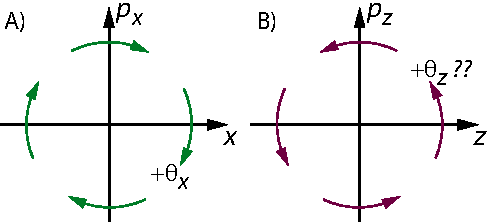
\includegraphics[width=5in]{tune.pdf}
  \caption[Illustration of a positive tune]{A) The standard accelerator physics convention is that 
a clockwise rotation in $(x, p_x)$ or $(y, p_y)$ space represents a positive tune. B) For longitudinal
oscillations, it is sometimes conventional to take counterclockwise rotation as positive if a machine
is always running above transition.}
  \label{f:tune}
\end{figure}

Given the $6 \times 6$ one-turn matrix for a storage ring, one issue is how to extract the tunes. If
there is no coupling the analysis is simple but with coupling things get more complicated. In the
general case, calculating with eigenvectors and eigenvalues gives, assuming that the lattice is
stable, three pairs of eigenvalues with the two eigenvalues of a given pair being complex
conjugates and all eigenvalues having unit amplitude. That is, the eigenvalues $\lambda_i$, $i =
1, \ldots 6$ can be ordered in pairs:
\begin{align}
  \lambda_1, \, \lambda_2 &= \exp(i \, \theta_a), \, \exp(-i \, \theta_a) \CRNO
  \lambda_3, \, \lambda_4 &= \exp(i \, \theta_b), \, \exp(-i \, \theta_b) \label{lleit} \\
  \lambda_5, \, \lambda_6 &= \exp(i \, \theta_c), \, \exp(-i \, \theta_c) \nonumber
\end{align}
where $\theta_a$, $\theta_b$, and $\theta_c$ are the three tunes. To associate $\lambda_1$ and
$\lambda_2$, along with their associated eigenvectors $\bfv_1$ and $\bfv_2$, with the
``horizontal-like'' mode, all the eigenvectors are compared to one another and the eigenvector pair
with the largest values for the $x$ and $p_x$ components are used for $\bfv_1$ and $\bfv_2$.
Similarly, for the ``vertical-like'' mode, eigenvector pair with the largest values for the $y$ and
$p_y$ components are associated with $\bfv_3$ and $\bfv_4$, and finally for the ``longitudinal-like''
mode the eigenvector pair with the largest values for the $z$ and $p_z$ components are associated
with $\bfv_5$ and $\bfv_6$.

It can be useful to arrange the eigenvalues such that the odd numbered eigenvalues (1, 3, and 5) are
associated with the tune and the even numbered eigen values (2, 4, and 6) are associated with the
negative of the tune as arranged in \Eq{lleit}. The algorithm for doing this can be deduced by first
considering the case where the motion is in one-dimension only. Here taken to be $(x, p)$ as shown
in \fig{f:tune}. Notice that, by the standard accelerator physics convention, a positive tune
represents a clockwise rotation in the transverse dimensions. For the longitudinal mode what counts
as positive tune can depend upon whether the machine is above transition or not. To keep the
mathematics consistent, positive tune for all modes will be taken to be clockwise.

Assuming that the motion is circular, the one-turn matrix $\bfM$ with tune $\theta$ is
\begin{equation}
  \bfM = \begin{pmatrix}
    \cos(\theta) & \sin(\theta) \\
   -\sin(\theta) & \cos(\theta)
  \end{pmatrix}
  \label{mctst}
\end{equation}
The eignvalues and eigenvectors are
\begin{alignat}{2}
  \lambda_1 &= \exp( i \, \theta),  \qquad &&\bfv_1 = \frac{1}{\sqrt{2}} \, (1, i) \CRNO
  \lambda_2 &= \exp(-i \, \theta),  \qquad &&\bfv_2 = \frac{1}{\sqrt{2}} \, (1, -i) 
\end{alignat}
Thus, for the eigenvector $(1, i)/\sqrt{2}$, were the momentum component is rotated by a factor
of $\pi/2$ counterclockwise from the position coordinate, the rotation angle is the tune. The
rotation angle associated with the eigenvector $(1, -i)/\sqrt{2}$ is associated with the negative of
the tune.

In the general case, each $\bfv_k$, $k = 1, \ldots 6$, is a vector in $(x, p_x, y, p_y, z, p_z)$
space with each component of the vector being a complex number. The criterion that an eigenvector
is associated with the tune is that the phase of the momentum components are on average rotated
clockwise from the position coordinates is
\begin{alignat}{2}
  \wt\bfv_{k}^* \, \bfS \, \bfv_k &=  i, \quad &&k = 1, 3, 5 \CRNO
  \wt\bfv_{k}^* \, \bfS \, \bfv_k &= -i, \quad &&k = 2, 4, 6
  \label{vsvi0}
\end{alignat}
where the tilde means transpose and $\bfS$ is the matrix
\begin{equation}
  \bfS = \begin{pmatrix}
      0 &  1 &  0 &  0 &  0 &  0 \\
     -1 &  0 &  0 &  0 &  0 &  0 \\
      0 &  0 &  0 &  1 &  0 &  0 \\
      0 &  0 & -1 &  0 &  0 &  0 \\
      0 &  0 &  0 &  0 &  0 &  1 \\
      0 &  0 &  0 &  0 & -1 &  0 \\
  \end{pmatrix}
  \label{s010000}
\end{equation}
\Eq{vsvi0}, along with the condition 
\begin{equation}
  v_{k+1} = v_k^*, \qquad k = 1, 3, 5
  \label{vv135}
\end{equation}
makes sure that the $\bfv_k$ are properly normalized.\footnote
  {
Different Authors use different conventions. For example, the $\bfS$ matrix in the paper by
Chao\cite{b:chao.spin}, is the negative of the $\bfS$ matrix defined here and in the paper by Ohmi,
Hirata, and Oide \cite{b:ohmi} the phases are reversed (positive phase is counterclockwise rotation)
as can be seen from Eqs.~(77) and (79) in their paper.
  }

%-----------------------------------------------------------------
\section{Linear Action-Angle Coordinates}
\label{s:action.ang}
\index{action-angle|hyperbf}

The transformation from the one-turn $6 \cross 6$ matrix $\bfT$ in laboratory coordinates to
action-angle coordinates uses the similarity transformation
\begin{equation}
  \bfT = \bfN \, \bfR \, \bfN^{-1}
\end{equation}
where $\bfN$ is a symplectic matrix. $\bfN^T \, \bfS \, \bfN = \bfS$ with $S$ given in \Eq{s010000}
and $\bfR$ is a rotation matrix
\begin{equation}
  \bfR = \begin{pmatrix}
    \bfR_2(\theta_a) &                  &                  \\
                     & \bfR_2(\theta_b) &                  \\
                     &                  & \bfR_2(\theta_c)
  \end{pmatrix}
\end{equation}
with each $2 \times 2$ rotation submatrix $\bfR_2$ being of the form as $\bfM$ in \Eq{mctst}.
The transformation from laboratory coordinates $\bfx$ to normal mode $\bfa$ coordinates is
\begin{equation}
  \bfa = \bfN^{-1} \, \bfx
\end{equation}
In action-angle coordinates $\bfa$ looks like
\begin{align}
  \bfa = &\left( \sqrt{2 \, J_a} \, \cos(\phi_a), -\sqrt{2 \, J_a} \, \sin(\phi_a), 
                 \sqrt{2 \, J_b} \, \cos(\phi_b), -\sqrt{2 \, J_b} \, \sin(\phi_b), \right. \\
        &\hskip20em \left. 
                 \sqrt{2 \, J_c} \, \cos(\phi_c), -\sqrt{2 \, J_c} \, \sin(\phi_c) 
         \right) \nonumber
\end{align}
where $J_a$, $J_b$, and $J_c$ are the actions and $\phi_a$, $\phi_b$, and $\phi_c$ are the angles.

When the motion is uncoupled, the action and angle of a mode is related to the laboratory coordinates, up
to an overall phase factor via:
\begin{align}
  x &= \sqrt{2 \, J \, \beta} \, \cos( \phi ) \CRNO
  p &= -\sqrt{\frac{2 \, J}{\beta}} \, \left( \alpha \, \cos( \phi ) + \sin( \phi ) \right) \CRNO
\end{align}

With the eigenvectors normalized with \Eq{vsvi0}, the particle position $\bfx$ on turn $m$ when a
single mode $k$ is excited can be written in the form
\begin{equation}
  \bfx(m) = \sqrt{J} \, \bfv_k \, e^{i \, (\theta_k \, m + \phi_0} + \text{C.C.}
  \label{x2jv}
\end{equation}
where the phase $\phi_0$ is set by the initial particle position $\bfx(0)$ and \vn{C.C.} means
complex conjugate.

The $\bfN$ matrix can be constructed using the eigenvectors of $\bfT$ (\sref{s:eigen.tune})
\begin{equation}
  \bfN = \frac{1}{\sqrt{2}} \, \left( 
    (\wt\bfv_1 + \wt\bfv_2), -i \, (\wt\bfv_1 - \wt\bfv_2), 
    (\wt\bfv_3 + \wt\bfv_4), -i \, (\wt\bfv_3 - \wt\bfv_4), 
    (\wt\bfv_5 + \wt\bfv_6), -i \, (\wt\bfv_5 - \wt\bfv_6)
  \right)
\end{equation}
where the tilde means transpose. That is, the $\wt\bfv_k$ are column vectors.

The $\bfv_k$ vectors, $k = 1, 3, 5$ can each be multiplied by an arbitrary complex phase factor $z$
with unit magnitude. The corresponding $\bfv_k$ must then be multiplied by $z^*$
to keep \Eq{vv135} satisfied. To recover the standard Twiss parameters, without coupling $\bfN$
should have the form
\begin{equation}
  \bfN = \begin{pmatrix}
    \bfN_a &        &        \\
           & \bfN_b &        \\
           &        & \bfN_c
  \end{pmatrix}
\end{equation}
where the $2 \times 2$ submatrices have the standard form
\begin{equation}
  \bfN_a = \begin{pmatrix}
    \sqrt{\beta_a}                                   & 0 \cr
    \frac{\tstyle -\alpha_a}{\tstyle \sqrt{\beta_a}} & \frac{\tstyle 1}{\tstyle \sqrt{\beta_a}}
  \end{pmatrix}
\end{equation}
with similar equations for $\bfN_b$ and $\bfN_c$. To make the $(1,2)$ component of these submatrices
zero, along with having $\sqrt{\beta}$ positive, the $k$\Th component of $\bfv_k$, $k = 1, 3, 5$
must be positive real. This fixes the overall phase of the eigenvectors.

%-----------------------------------------------------------------
\section{Dispersion Calculation}
\label{s:dispersion}
\index{dispersion|hyperbf}

The dispersion ($\eta$) and the dispersion derivative ($\eta'$) are defined by the equations
\begin{align}
  \eta_x(s) &\equiv \left. \frac{dx}{dp_z} \right|_s \comma \qquad
    \eta'_x(s) \equiv \left. \frac{d\eta_x}{ds} \right|_s
    = \left. \frac{dx'}{dp_z} \right|_s \CRNO
  \eta_y(s) &\equiv \left. \frac{dy}{dp_z} \right|_s \comma \qquad
    \eta'_y(s) \equiv \left. \frac{d\eta_y}{ds} \right|_s
    = \left. \frac{dy'}{dp_z} \right|_s \\
  \eta_z(s) &\equiv \left. \frac{dz}{dp_z} \right|_s \nonumber
\end{align}

Given the dispersion at a given point, the dispersion at some other point is calculated as follows:
Let $\Bf r = (x, p_x, y, p_y, z, p_z)$ be the reference orbit, around which the dispersion is to be
calculated. Let $\bfV$ and $\bf M$ be the zeroth and first order components of the transfer map
between two points labeled 1 and 2:
\begin{equation}
  \Bf r_2 = \bfM \, \Bf r_1 + \bfV
  \label{rmrv}
\end{equation}
Define the dispersion vector $\bfeta$ by
\begin{equation}
  \bfeta = 
  \left( 
    \eta_x, \eta'_x \, (1 + p_z), \eta_y, \eta'_y \, (1 + p_z), \eta_z, 1
  \right)
\end{equation}
Differentiating \Eq{rmrv} with respect to energy, the dispersion at point 2 in terms of the
dispersion at point 1 is
\begin{equation}
  \bfeta_2 = \left[ \frac{dp_{z2}}{dp_{z1}} \right]^{-1} \, 
    \left[ \bfM \, \bfeta_1 \right] + \bfV_\eta 
    \label{eppmev}
\end{equation}
where
\begin{equation}
  \bfV_\eta = \left[ \frac{dp_{z2}}{dp_{z1}} \right]^{-1} \, 
  \frac{1}{1 + p_{z1}}
  \left(
  \begin{array}{c}
    M_{12} \, p_{x1} + M_{14} \, p_{y1} \\
    M_{22} \, p_{x1} + M_{24} \, p_{y1} \\
    M_{32} \, p_{x1} + M_{34} \, p_{y1} \\
    M_{42} \, p_{x1} + M_{44} \, p_{y1} \\
    M_{52} \, p_{x1} + M_{54} \, p_{y1} \\
    M_{62} \, p_{x1} + M_{64} \, p_{y1} \\
  \end{array}
  \right)
  -
  \left(
  \begin{array}{c}
    0 \\
    \frac{p_{x2}}{1 + p_{z2}} \\
    0 \\
    \frac{p_{y2}}{1 + p_{z2}} \\
    0 \\
    0 
  \end{array}
  \right)
\end{equation}
The sixth row of the matrix equation gives $dp_{z1}/dp_{z2}$. 
Explicitly
\begin{equation}
  \frac{dp_{z2}}{dp_{z1}} =
  \sum_{i=1}^6 M_{6i} \, \eta_{1i} + 
  \frac{M_{62} \, p_{x1} + M_{64} \, p_{y1}}{1 + p_{z1}}
\end{equation}
For everything except \vn{RFcavity} and \vn{Lcavity} elements, 
$dp_{z2}/dp_{z1}$ is 1.

For a non-circular machine, there are two ways one can imagine defining the dispersion: Either with
respect to changes in energy at the beginning of the machine or with respect to the local change in
energy at the point of measurement. The former definition will be called ``non-local dispersion''
and the latter definition will be called ``local dispersion''. For a circular machine, local
dispersion is always used.  The dispersion defined in the above equations, which is what \bmad uses
in calculations, is the local dispersion. The non-local dispersion $\wt\bfeta(s_1)$ at some point
$s_1$ is related to the local dispersion $\bfeta(s_1)$ via
\begin{equation}
  \wt\bfeta(s_1) = \frac{dp_{z1}}{dp_{z0}} \, \bfeta(s_1)
\end{equation}
where $s_0$ is the beginning of the machine.

For a non-circular machine, there are advantages and disadvantages to using either local or
non-local dispersion. Local dispersion has the problem that $dp_{z2}/dp_{z1}$ in \Eq{eppmev} may go
through zero at a point producing infinite dispersions at that point. The non-local dispersion has
the merit of reflecting what one would measure if the starting energy of the beam is varied. The
local dispersion, on the other hand, reflects the correlations between the particle energy and
particle position within a beam.

